\chapter{Implementeren van een chatfrontend}
Nu we de backend hebben voor onze digitale assistent, is het tijd om er een aantrekkelijke, overzichtelijke en snelle frontend interface aan te verbinden. 
Er zijn heel veel frontend libraries die via NodeJS, Deno, Bun en andere JavaScript frameworks kunnen gedeployed worden in een paar seconden. 

In dit voorbeeld zullen we een template gebruiken van NextJS en aanpassen naar onze wens. 
Het voordeel hier is dat we geen tijd moeten spenderen aan het bouwen van een interface omdat we al een mooie, overzichtelijke interface hebben. Deze ziet er uit als onderstaande screenshot:

\begin{figure}[h]
	\makebox[\textwidth]{
		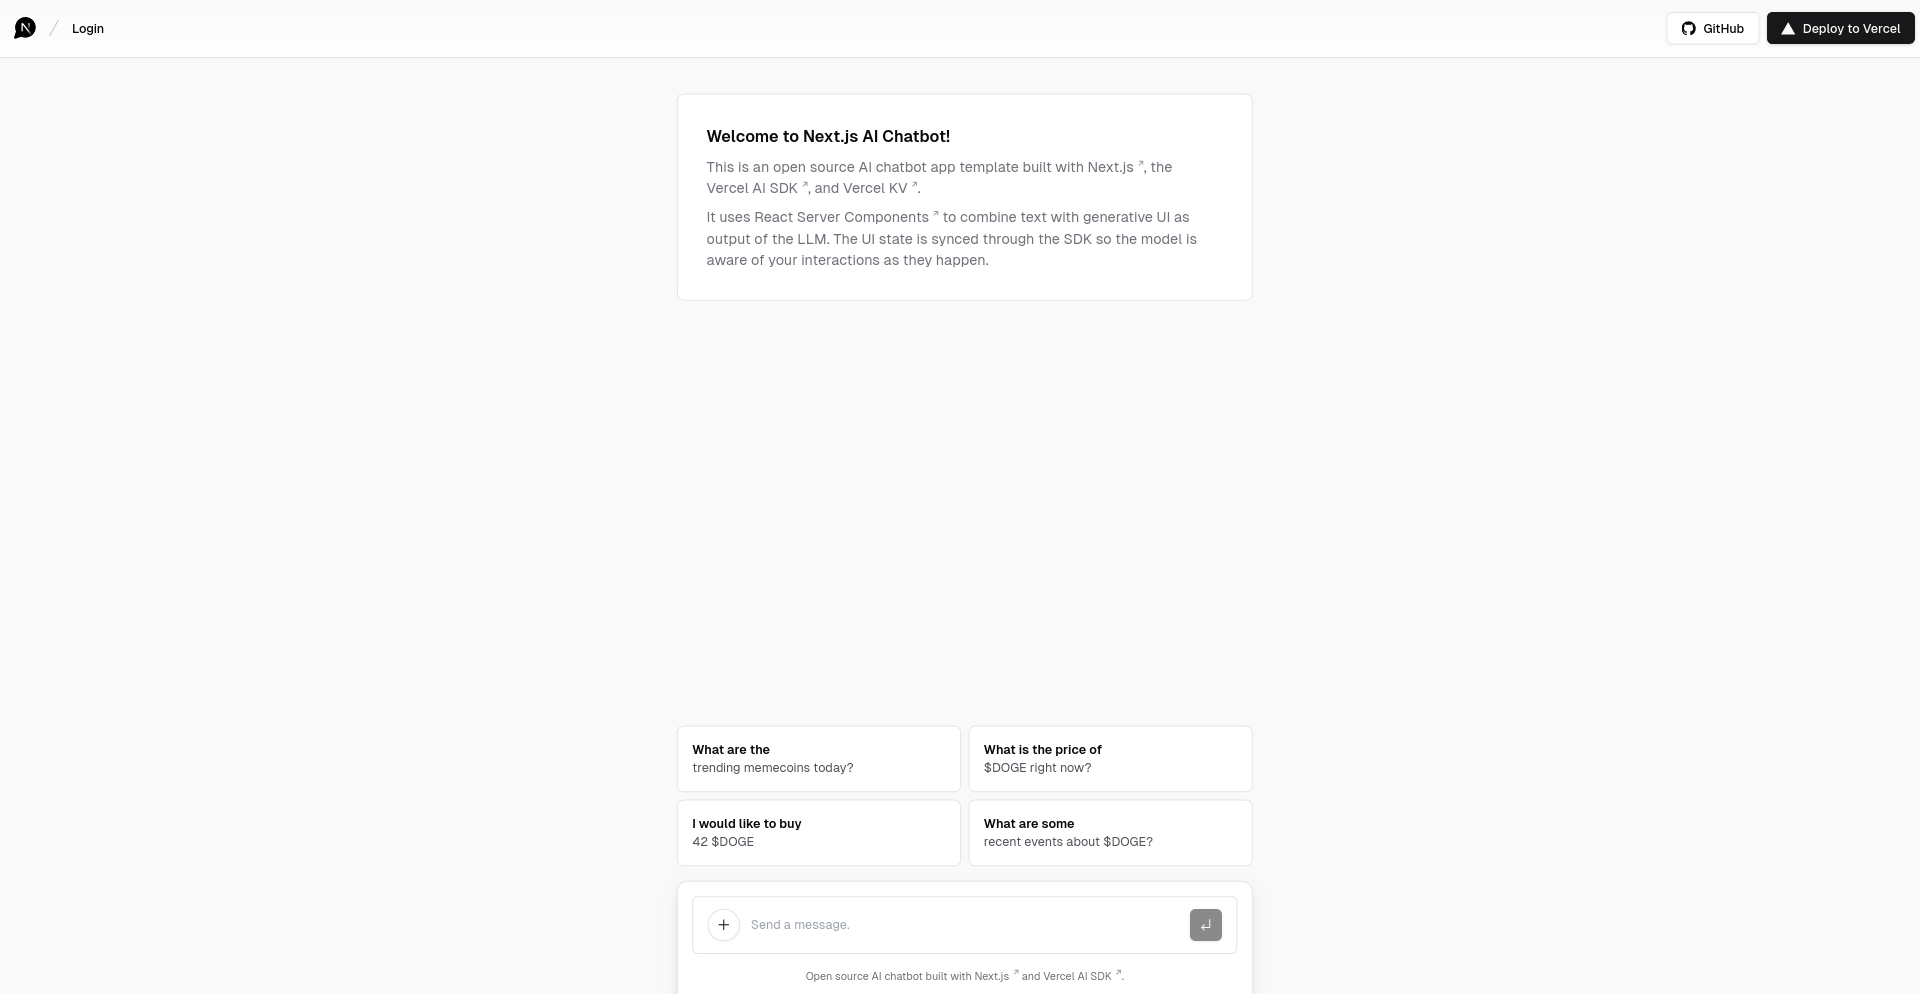
\includegraphics[width=\textwidth]{chat_frontend.png}
	}
	\captionof{figure}{Screenshot van NextJS template chat frontend}
\end{figure}
\newpage

Deze chatbot komt standaard met OpenAI API ingebouwd. 
Er zal dus wat sleutelwerk nodig zijn om deze te linken met onze Ollama interne API, maar de open-source strategie van deze chatapp maakt ons dit gelukkig vrij gemakkelijk. 
NodeJS maakt het ons ook makkelijk om op een lokale machine bij Deltalex te deployen. 
Op deze manier kunnen we het volledige systeem isoleren en lokaal houden, om het zo veilig mogelijk te houden. 

Het nadeel van deze lokale aanpak is dat er een sterke grafische kaart in de lokale machine moet zitten om modellen performant te kunnen draaien voor meerdere gebruikers op hetzelfde tijdstip. 
Daarom is deze paper slechts een roadmap die de lezer tot een volledige, werkelijke implementatie leidt. 
